%%%%%%%%%%%%%%%%%%%%%%%%%%%%%%%%%%%%%%%%%%%%%%%%%%%%%%%%%%%%%%%%%%%%%%%%%%%%%%%%%%%%%%%%%%%%
%%
%% Chapter 1 : Introduction
%%
%%      * Should give an intro/overview of the problem and the context in which it arises
%%      * Then, it should emphasize the problem (problem statement)
%%      * Then the objectives of the proposed research topic and problem
%%      * And finally the organization/structure of the document
%%
%%%%%%%%%%%%%%%%%%%%%%%%%%%%%%%%%%%%%%%%%%%%%%%%%%%%%%%%%%%%%%%%%%%%%%%%%%%%%%%%%%%%%%%%%%%%
\chapter{Introduction}
\label{ch:intro}

%%%%%%%%%%%%%%%%%%%%%%%%%%%%%%%
%   Figures for chapter 1
%%%%%%%%%%%%%%%%%%%%%%%%%%%%%%%

\newcommand{\figDrlLocomotionMotivation}{
    \begin{figure}[!ht]
        \centering
        \begin{subfigure}[b]{0.45\textwidth}
            \centering
            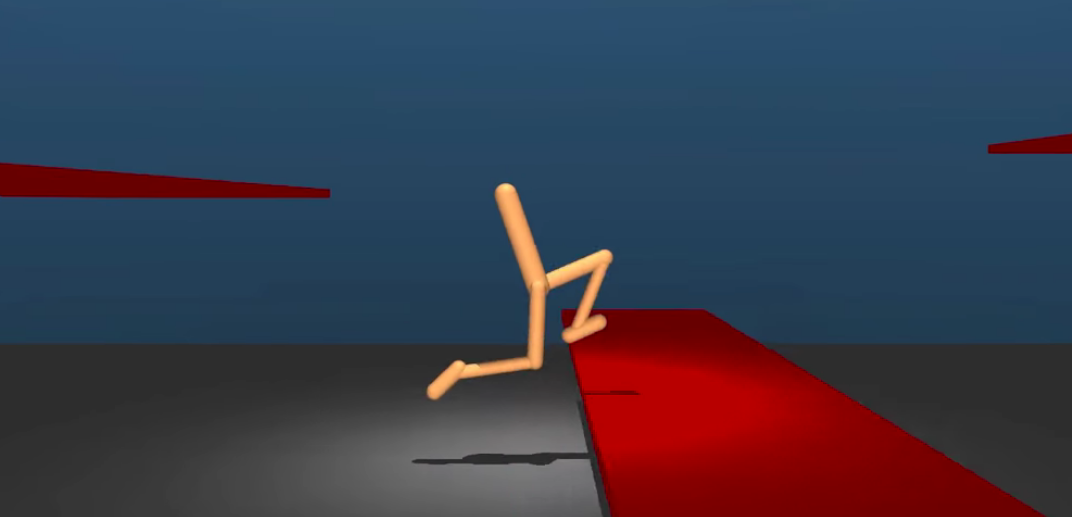
\includegraphics[width=0.9\textwidth]{./chapters/chapter_1/imgs/img_ch1_emergence_of_locomotion.png}
            \caption{}
            \label{fig:ch1_emergence_locomotion}
        \end{subfigure}
        \begin{subfigure}[b]{0.45\textwidth}
            \centering
            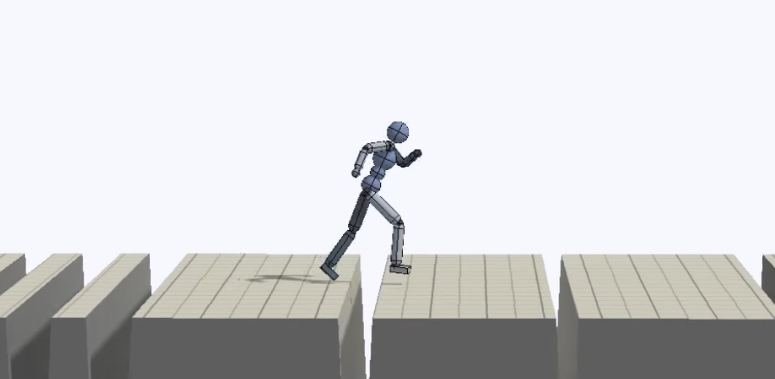
\includegraphics[width=0.9\textwidth]{./chapters/chapter_1/imgs/img_ch1_deepmimic.png}
            \caption{}
            \label{fig:ch1_deepmimic}
        \end{subfigure}
        \caption{Some results from applying Deep Reinforcement Learning to locomotion. 
                    a) Biped traversing simulated environment \citep{DeepmindEmergenceLocomotion}.
                    b) Humanoid traversing simulated environment \citep{DeepMimic} }
        \label{fig:ch1_motivation_drl_locomotion}
    \end{figure}
}

\newcommand{\figDrlBenchmarks}{
    \begin{figure}
        %% Controlsuite
        \centering
        \begin{subfigure}[b]{1.0\textwidth}
            \centering
            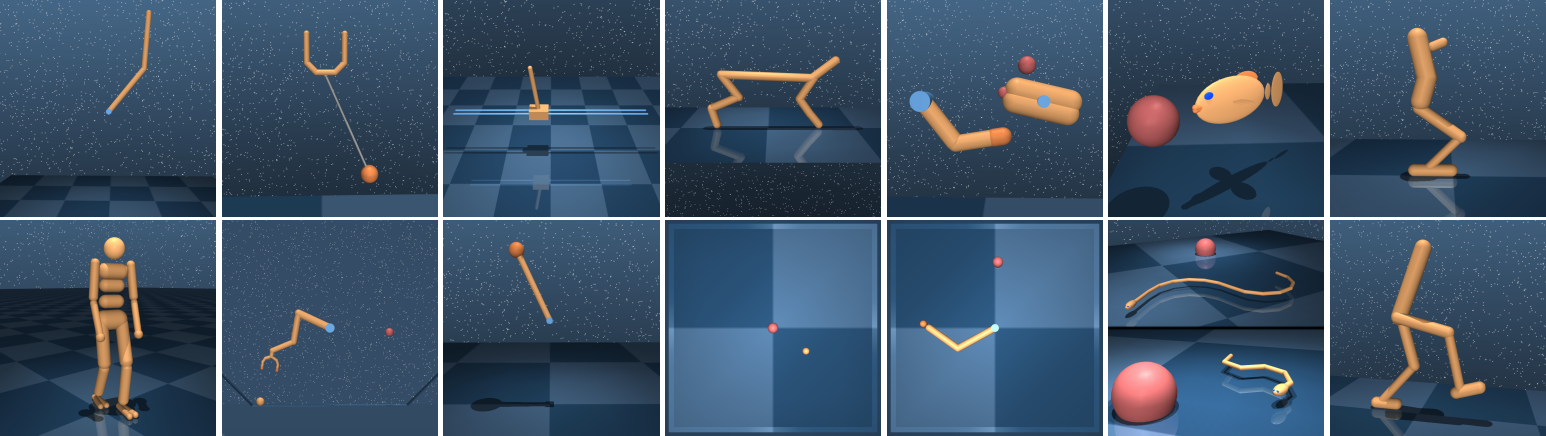
\includegraphics[width=1.0\textwidth]{./chapters/chapter_1/imgs/img_ch1_benchmarks_controlsuite.png}
            \caption{}
            \label{fig:ch1_benchmarks_controlsuite}
        \end{subfigure}
        %% Roboschool
        \centering
        \begin{subfigure}[b]{1.0\textwidth}
            \centering
            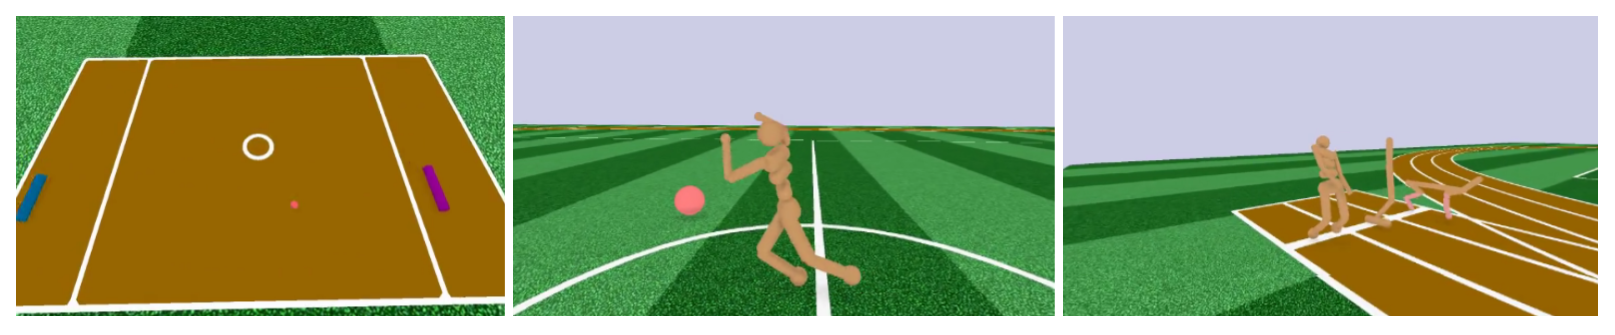
\includegraphics[width=1.0\textwidth]{./chapters/chapter_1/imgs/img_ch1_benchmarks_roboschool.png}
            \caption{}
            \label{fig:ch1_benchmarks_roboschool}
        \end{subfigure}
        %% Gym
        \centering
        \begin{subfigure}[b]{1.0\textwidth}
            \centering
            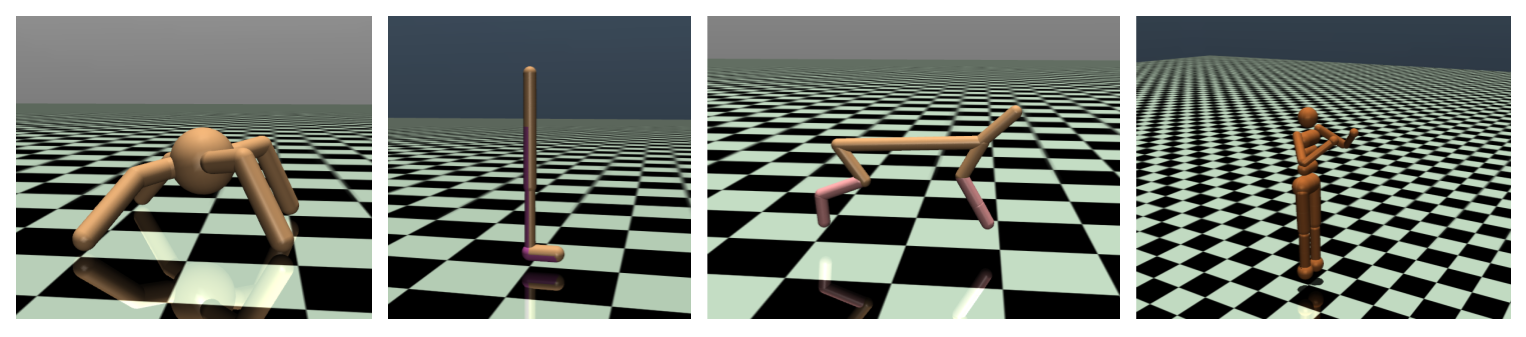
\includegraphics[width=1.0\textwidth]{./chapters/chapter_1/imgs/img_ch1_benchmarks_gym.png}
            \caption{}
            \label{fig:ch1_benchmarks_gym}
        \end{subfigure}
        %% Rllab
        \centering
        \begin{subfigure}[b]{1.0\textwidth}
            \centering
            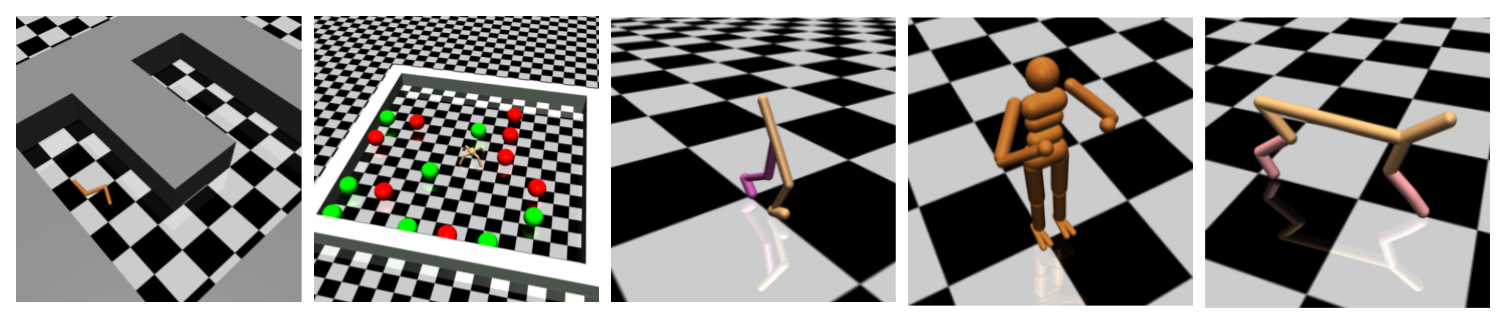
\includegraphics[width=1.0\textwidth]{./chapters/chapter_1/imgs/img_ch1_benchmarks_rllab.png}
            \caption{}
            \label{fig:ch1_benchmarks_rllab}
        \end{subfigure}
        \caption{Available benchmarks for locomotion tasks: 
                            a) controlsuite \citep{Controlsuite},
                            b) roboschool \citep{Roboschool},
                            c) gym \citep{Gym} and
                            d) rllab \citep{Rllab}}
        \label{fig:ch1_drl_locomotion_benchmarks}
    \end{figure}
}

\newcommand{\figEnvironmentsProposalFromTo}{
    \begin{figure}
        \centering
        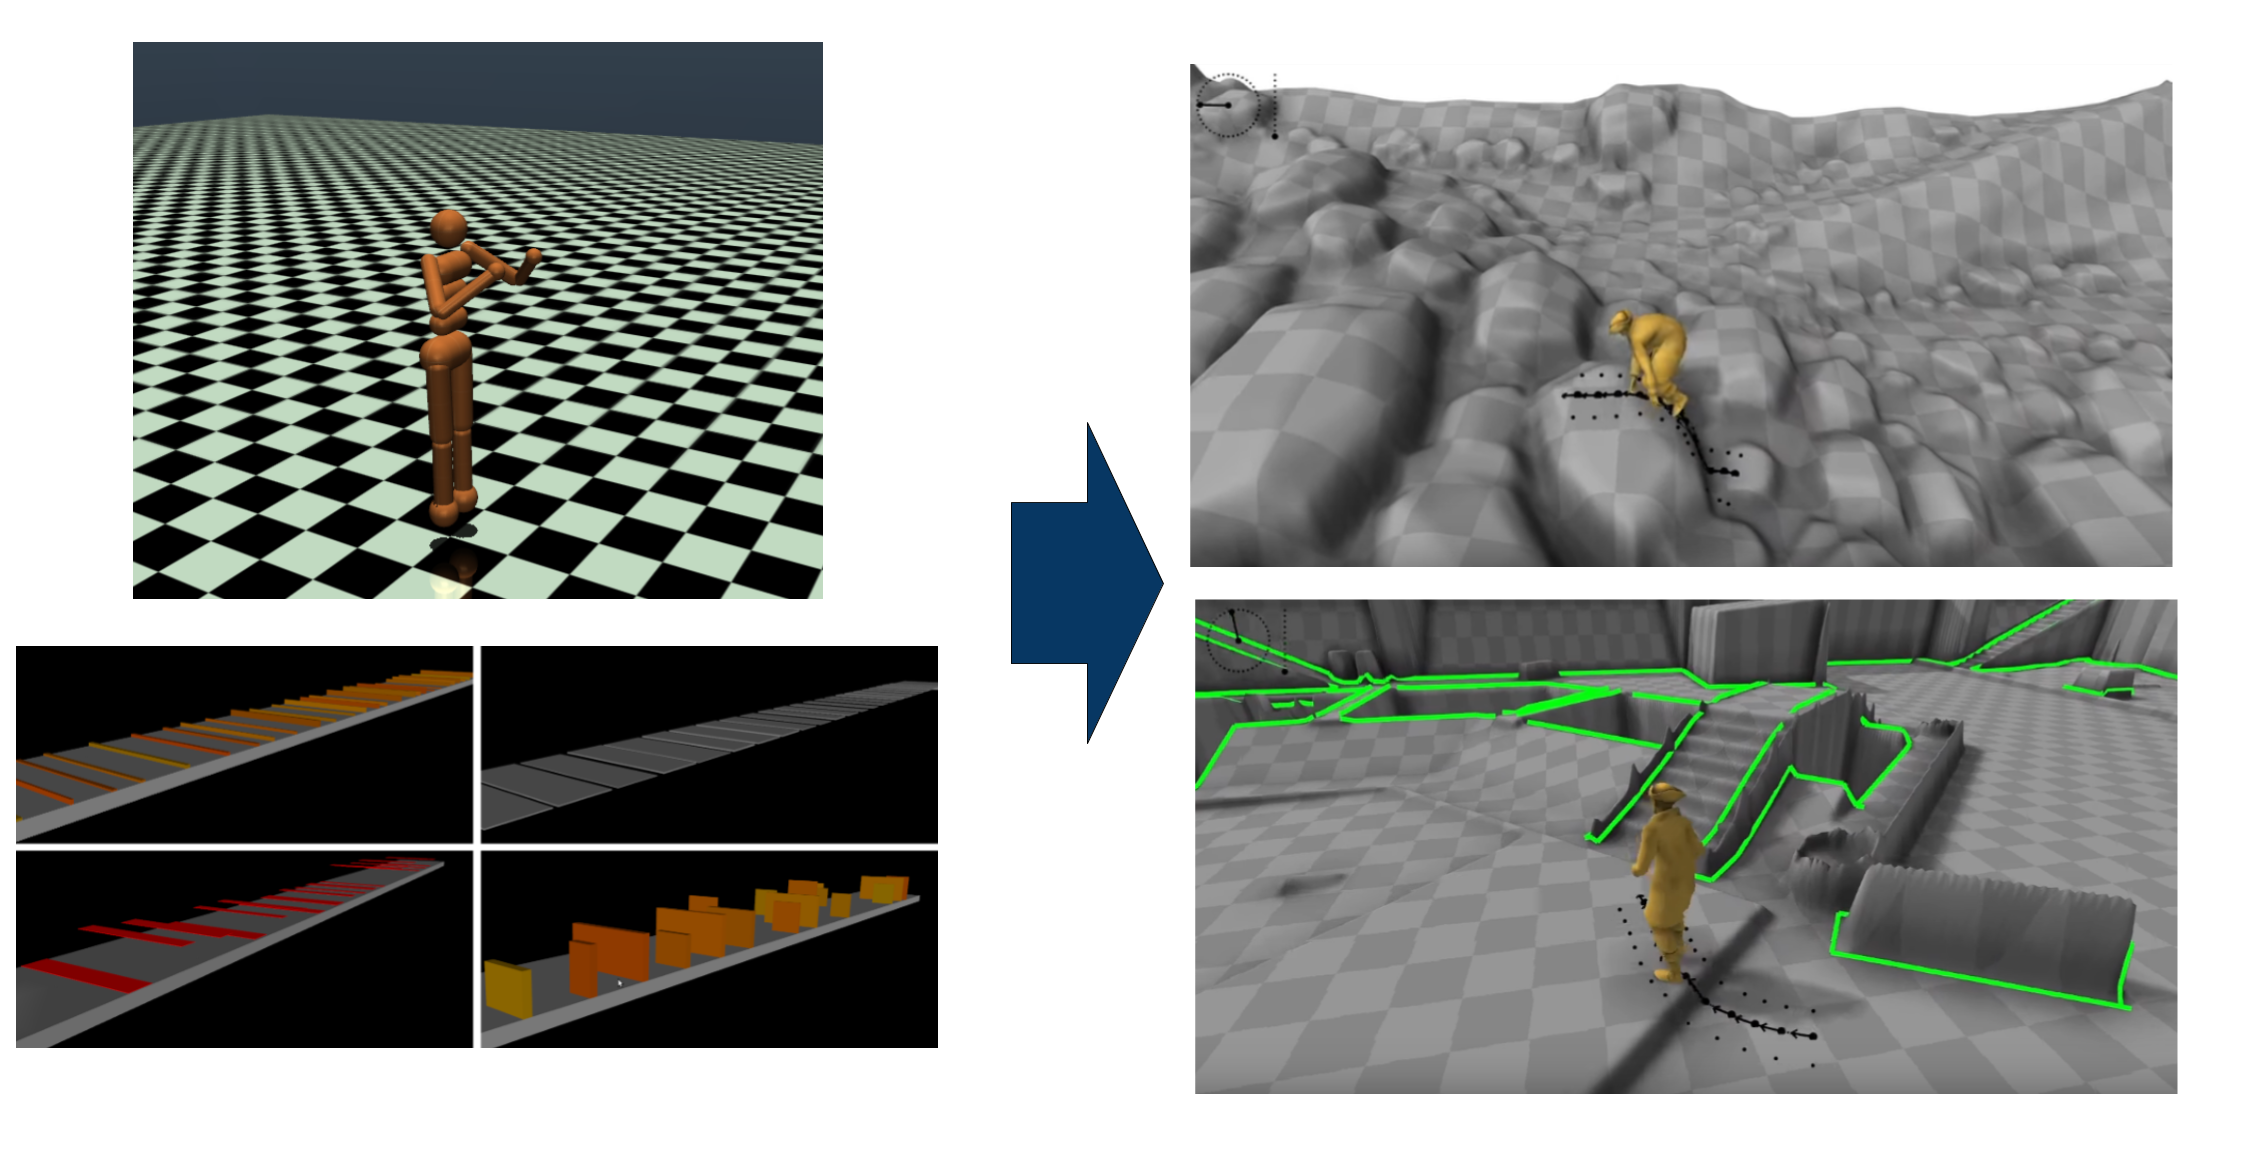
\includegraphics[width=0.8\textwidth]{./chapters/chapter_1/imgs/img_ch1_environments_from_to.png}
        \caption{Comparison of the proposed environments to the environments provided by current benchmarks. 
                 Left: relatively simple environments (image adapted from \citet{Gym}). 
                 Right: relatively more complex proposed environments (images adapted from \citet{Pfnn} ).}
        \label{fig:ch1_environments_comparison_from_to}
    \end{figure}
}

\newcommand{\figEnvManipSimToreal}{
    \begin{figure}
        \centering
        \begin{subfigure}[b]{0.5\textwidth}
            \centering
            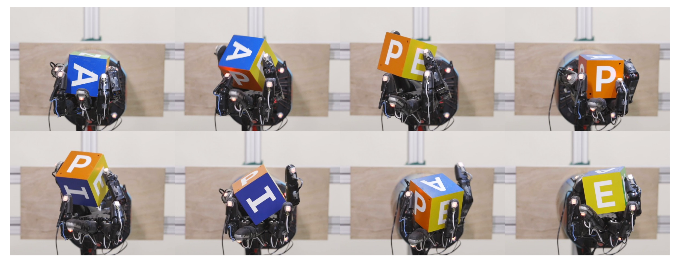
\includegraphics[width=1.0\textwidth]{./chapters/chapter_1/imgs/img_ch1_openai_robot_dexterity.png}
            \caption{}
            \label{fig:ch1_openai_robot_dexterity}
        \end{subfigure}
        \begin{subfigure}[b]{0.5\textwidth}
            \centering
            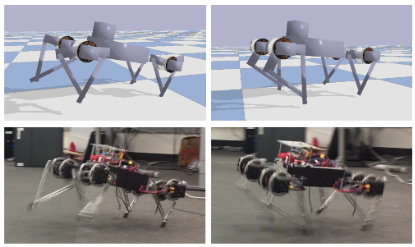
\includegraphics[width=1.0\textwidth]{./chapters/chapter_1/imgs/img_ch1_google_brain_minitaur_sim_to_real.png}
            \caption{}
            \label{fig:ch1_google_brain_minitaur_sim_to_real}
        \end{subfigure}
        \caption{Some examples of sim2real results: 
                            a) Robotic hand generalizing in randomized environment \citep{OpenAISim2real}.
                            b) Quadruped trained in simulation and deployed in real world \citep{GoogleBrainSim2Real} }
        \label{fig:ch1_sim_to_real_approaches}
    \end{figure}
}

Recent advances in the field of Deep Reinforcement Learning (DRL) have achieved impressive
results in various complex tasks, like being able to play Atari games at a super human level \citep{DQNAtari}, 
and beating the world's Go champion \citep{AlphaGo}, just to name a few. These represent discrete 
action spaces problems, in which the action space can be defined by a finite-size set of values. 
More recently, this approach has also been applied to continuous actions spaces, i.e. in continuous 
control tasks. This has given good results in various locomotion benchmarks, like in 
\citeauthor{DeepmindEmergenceLocomotion} and \citeauthor{DeepMimic}, shown in Figure @FIG-1.1.

\figDrlLocomotionMotivation

This approach is very promising because it allows an agent to learn an appropriate controller for a given task after training in
the simulated environment, which reduces the need to implement highly sophisticated control pipelines. Currently available 
training environments have been presented in various articles, and we will talk more about these in Chapter 3.
Some of these training environments are shown in Figure @FIG-1.2.

%% and compared to the ones mentioned previously (from Figure @FIG-1.1)
%%they are much simpler, consisting mostly of classic control problems and some locomotion tasks in flat terrains.

The ultimate goal of applying these techniques is to be able to develop complex behaviours, similar
to those shown in nature by animals. However, to develop and test this complex behaviours there is a need to \textbf{create
a wide set of rich and complex environments}, which is not provided by currently available locomotion benchmarks.

\figDrlBenchmarks

% @TAG: Refer to content above and "formalize" a bit more
\section{Problem Statement}
\label{sec:problem}

As explained previously, currently there are no robot locomotion benchmarks that allow
to \textbf{create diverse learning environments}, which limits the range of behaviours that can be learned
from scratch using Deep Reinforcement Learning techniques. Besides, there are some other issues 
that arise in the context of learning locomotion behaviours:

\begin{itemize}
	\item \textbf{Exploitation} of the dynamics of the simulated environments: 
			Because of the nature of the objective the agents try to optimize for, they usually
			end up developing behaviours that cheat by exploiting some specific aspects of the environment
			and getting stuck sub-optimal behaviours, e.g. walking in very unnatural way in walking tasks.
			This is specially true when designing a reward function. The reward is the signal
			that the agent gets to improve its behaviours, so poorly engineered reward functions could lead to sub-optimal and even bad performance.
	\item \textbf{Inability to transfer} learned  policies into the real world:
			In general, policies learned in simulation do not transfer directly to a real world robotics
			platform. This is because of discrepancies between the dynamics of the simulation and
			the dynamics of the real world, which is usually called the \textbf{reality gap}.
			This issue is also a direct consequence of the previous one. As the agent exploits the 
			dynamics of the simulation, it will overfit to the given environment, and will 
			not generalize when transferred to the real world.
\end{itemize}

Some approaches used to deal with these issues are related to controlling the learning 
environments itself, like in \citeauthor{GoogleBrainSim2Real} and \citeauthor{OpenAISim2real} (Figure @FIG-1.3). 
These try to account for unmodeled dynamics and generalization by using randomization
over the simulated environment and other techniques to force the learning agent not to 
overfit to a specific behaviour that only exploits some of the dynamics of the environment.

Then, one approach that can be used to solve these issues is to have a framework
that provides researchers with the tools required to create these diverse environments
and have full control over them. Furthermore, such a framework could be used to develop
environments in a progressive way via a \textbf{curriculum} (proposed in @CITE). Based on
all this, we formulate the following hypothesis:

\begin{hypothesis}
	By having control of the learning environment we can control the learning procedure
	of an agent in such a way that it can develop complex and robust behaviours to solve
	the tasks presented, and also generalize to other environments.
\end{hypothesis}

We will focus in testing half of this hypothesis by implementing the required framework
to create these diverse environments, and evaluating current state of the art Deep RL algorithms
to these new environments. As future work we will try to deal with the full hypothesis, by
trying to develop appropriate curricula.

\figEnvManipSimToreal

\figEnvironmentsProposalFromTo

% @TAG: Refer to initial content and "emphazise" the objectives
\section{Objectives}
\label{sec:objectives}

\subsection*{General Objective}
Develop a framework that allows the creation of diverse learning environments for locomotion tasks (as shown in Figure @FIG-1.4), 
and evaluate the performance and generalization capabilities of current state of the art Deep 
Reinforcement Learning algorithms.
\todo{redacta mejor el objetivo, make y build tienen significados similares, tal vez sea mejor develop a framework that allow us to build...}

\subsection*{Specific Objectives}
\begin{itemize}
 \item Implement an abstract core framework for robot locomotion, decoupled from any
       concrete physics engine currently available.
 \item Implement wrapper functionality for the integration of various 
       currently available physics engines following a common API.
 \item Implement a set of APIs that allows to create diverse and complex
       environments, and create diverse tasks using these environments.
 \item Implement user APIs via Python bindings to allow users to easily interact
       with the framework, set up experiments and train agents using current Deep Learning Frameworks.
 \item Make the necessary documentation for the whole framework to allow further
       development of this framework and adoption as a standardized benchmark 
       for robot locomotion.
 \item Evaluate the performance of state of the art Deep Reinforcement Learning algorithms
       in these environments.
\end{itemize}
\todo{solo hay dos objetivos específicos?}

\section{Organization}
\label{sec:organization}

The structure of this proposal is as follows :

\begin{itemize}
	\item \textbf{Chapter 2 - Related background}: we present the necessary background and
		  terminology used throught this document.
	\item \textbf{Chapter 3 - Related works}: we discuss the currently available benchmarks by
		  analyzing the provided functionality and use cases. We also discuss some
		  state of the art algorithms used with these benchmarks, which will be
		  implemented and evaluated with the proposed framework.
	\item \textbf{Chapter 4 - Proposal in depth}: we discuss more details of the proposed framework,
		  including: architecture of the framework, core features to be implemented, etc.
	\item \textbf{Chapter 5 - Current progress}: we discuss the current state of the implementation
		  of the proposed framework.
    \item \textbf{Chapter 6 - Discussion}: finally, in this chapter we present
          a discussion on the whole proposal and the road-map that we are 
          following towards the objectives proposed earlier.
		  
		  \todo{Seria bueno un capítulo de conclusiones}
		 
\end{itemize}